\documentclass{article}
\usepackage{amsmath}
\usepackage{graphicx}
\usepackage{listings}
\usepackage{xcolor}
\usepackage{float}
% \usepackage[bahasa]{babel}

\usepackage{titling}
\setlength{\droptitle}{-4em}   % Adjust this value as needed
\usepackage{subcaption}

\lstdefinestyle{python}{
  language=Python,
  basicstyle=\ttfamily\small,
  numberstyle=\tiny\color{gray},
  numbers=left,
  numbersep=5pt,
  showstringspaces=false,
  breaklines=true,
  frame=single,
  frameround=tttt,
  backgroundcolor=\color{gray!5},
  commentstyle=\color{green!60!black}\itshape,
  keywordstyle=\color{blue!80!black}\bfseries,
  stringstyle=\color{red!70!black},
  emphstyle=\color{purple!70!black}\bfseries,
  emph={import,from,as,def,class,if,elif,else,for,while,with,try,except,finally,return,yield,lambda,True,False,None},
  morekeywords={self,numpy,matplotlib,pyplot,signal,deque,threading,queue,serial},
  captionpos=b,
  aboveskip=1.5\baselineskip,
  belowskip=1.5\baselineskip,
  columns=flexible,
  keepspaces=true,
  tabsize=4,
  xleftmargin=10pt,
  xrightmargin=10pt
}
\lstdefinestyle{vhdl}{
  language=VHDL,
  basicstyle=\ttfamily\footnotesize,
  numberstyle=\tiny,
  numbers=left,
  numbersep=5pt,
  showstringspaces=false,
  breaklines=true,
  frame=single,
  backgroundcolor=\color{gray!5},
  commentstyle=\color{green!60!black},
  keywordstyle=\color{blue!80!black},
  stringstyle=\color{purple!40!black}
}

\usepackage[top=2cm, bottom=2cm, left=2.5cm, right=2.5cm]{geometry}

\begin{document}

\title{Laporan Final Project PKT: Implementasi HPF FIR pada FPGA DE-10 Lite}
\author{Figo Arzaki Maulana - 5022221041}
\date{Rabu, 26 Juni 2025}
\maketitle

\section{Pendahuluan}

Final project ini bertujuan untuk merancang dan mengimplementasikan filter FIR (Finite Impulse Response)
jenis high-pass pada platform FPGA DE-10 Lite menggunakan bahasa VHDL dan dirancang dengan metode windowing Hamming.
Sistem yang dikembangkan mampu memproses sinyal analog dengan bandwidth 10 kHz melalui ADC 12-bit,
kemudian menerapkan filtering digital dengan frekuensi cut-off 1100 Hz yang dihitung berdasarkan formula $1000 + (\text{angka NRP terakhir} \times 100)$ Hz.
Sistem dilengkapi dengan komunikasi UART untuk mentransmisikan data hasil filtering ke komputer,
dimana sinyal ditampilkan dalam bentuk grafik menggunakan Python matplotlib.

Proyek ini mendemonstrasikan implementasi lengkap sistem pemrosesan sinyal digital pada FPGA,
mulai dari akuisisi data analog, pemrosesan digital real-time, hingga visualisasi hasil untuk validasi
performa filter yang telah dirancang.

\section{Metodologi}

\subsection{Sampling Sinyal Analog}
Sinyal analog diambil menggunakan ADC 12-bit yang terhubung ke FPGA DE-10 Lite.
ADC ini beroperasi pada frekuensi sampling 25 kHz yang didapat dari mendesimasi clock 50MHz.
Pada implementasinya ADC ini menggunakan modul IP ADC
yang telah tersedia pada Quartus.

\subsection{Desain Filter FIR}
Filter FIR dirancang menggunakan metode windowing Hamming menggunakan kode Python berikut:
\begin{lstlisting}[style=python]
fir_coefficients = signal.firwin(filter_order, normalized_cutoff, window='hamming', pass_zero='highpass')
\end{lstlisting}
Dengan orde filter berjumlah 51 dan frekuensi cut-off 1100 Hz yang dinormalisasi terhadap frekuensi Nyquist (12.5 kHz).
Respon frekuensi yang didapatkan dari desain filter ini adalah sebagai berikut:
\begin{figure}[H]
  \centering
  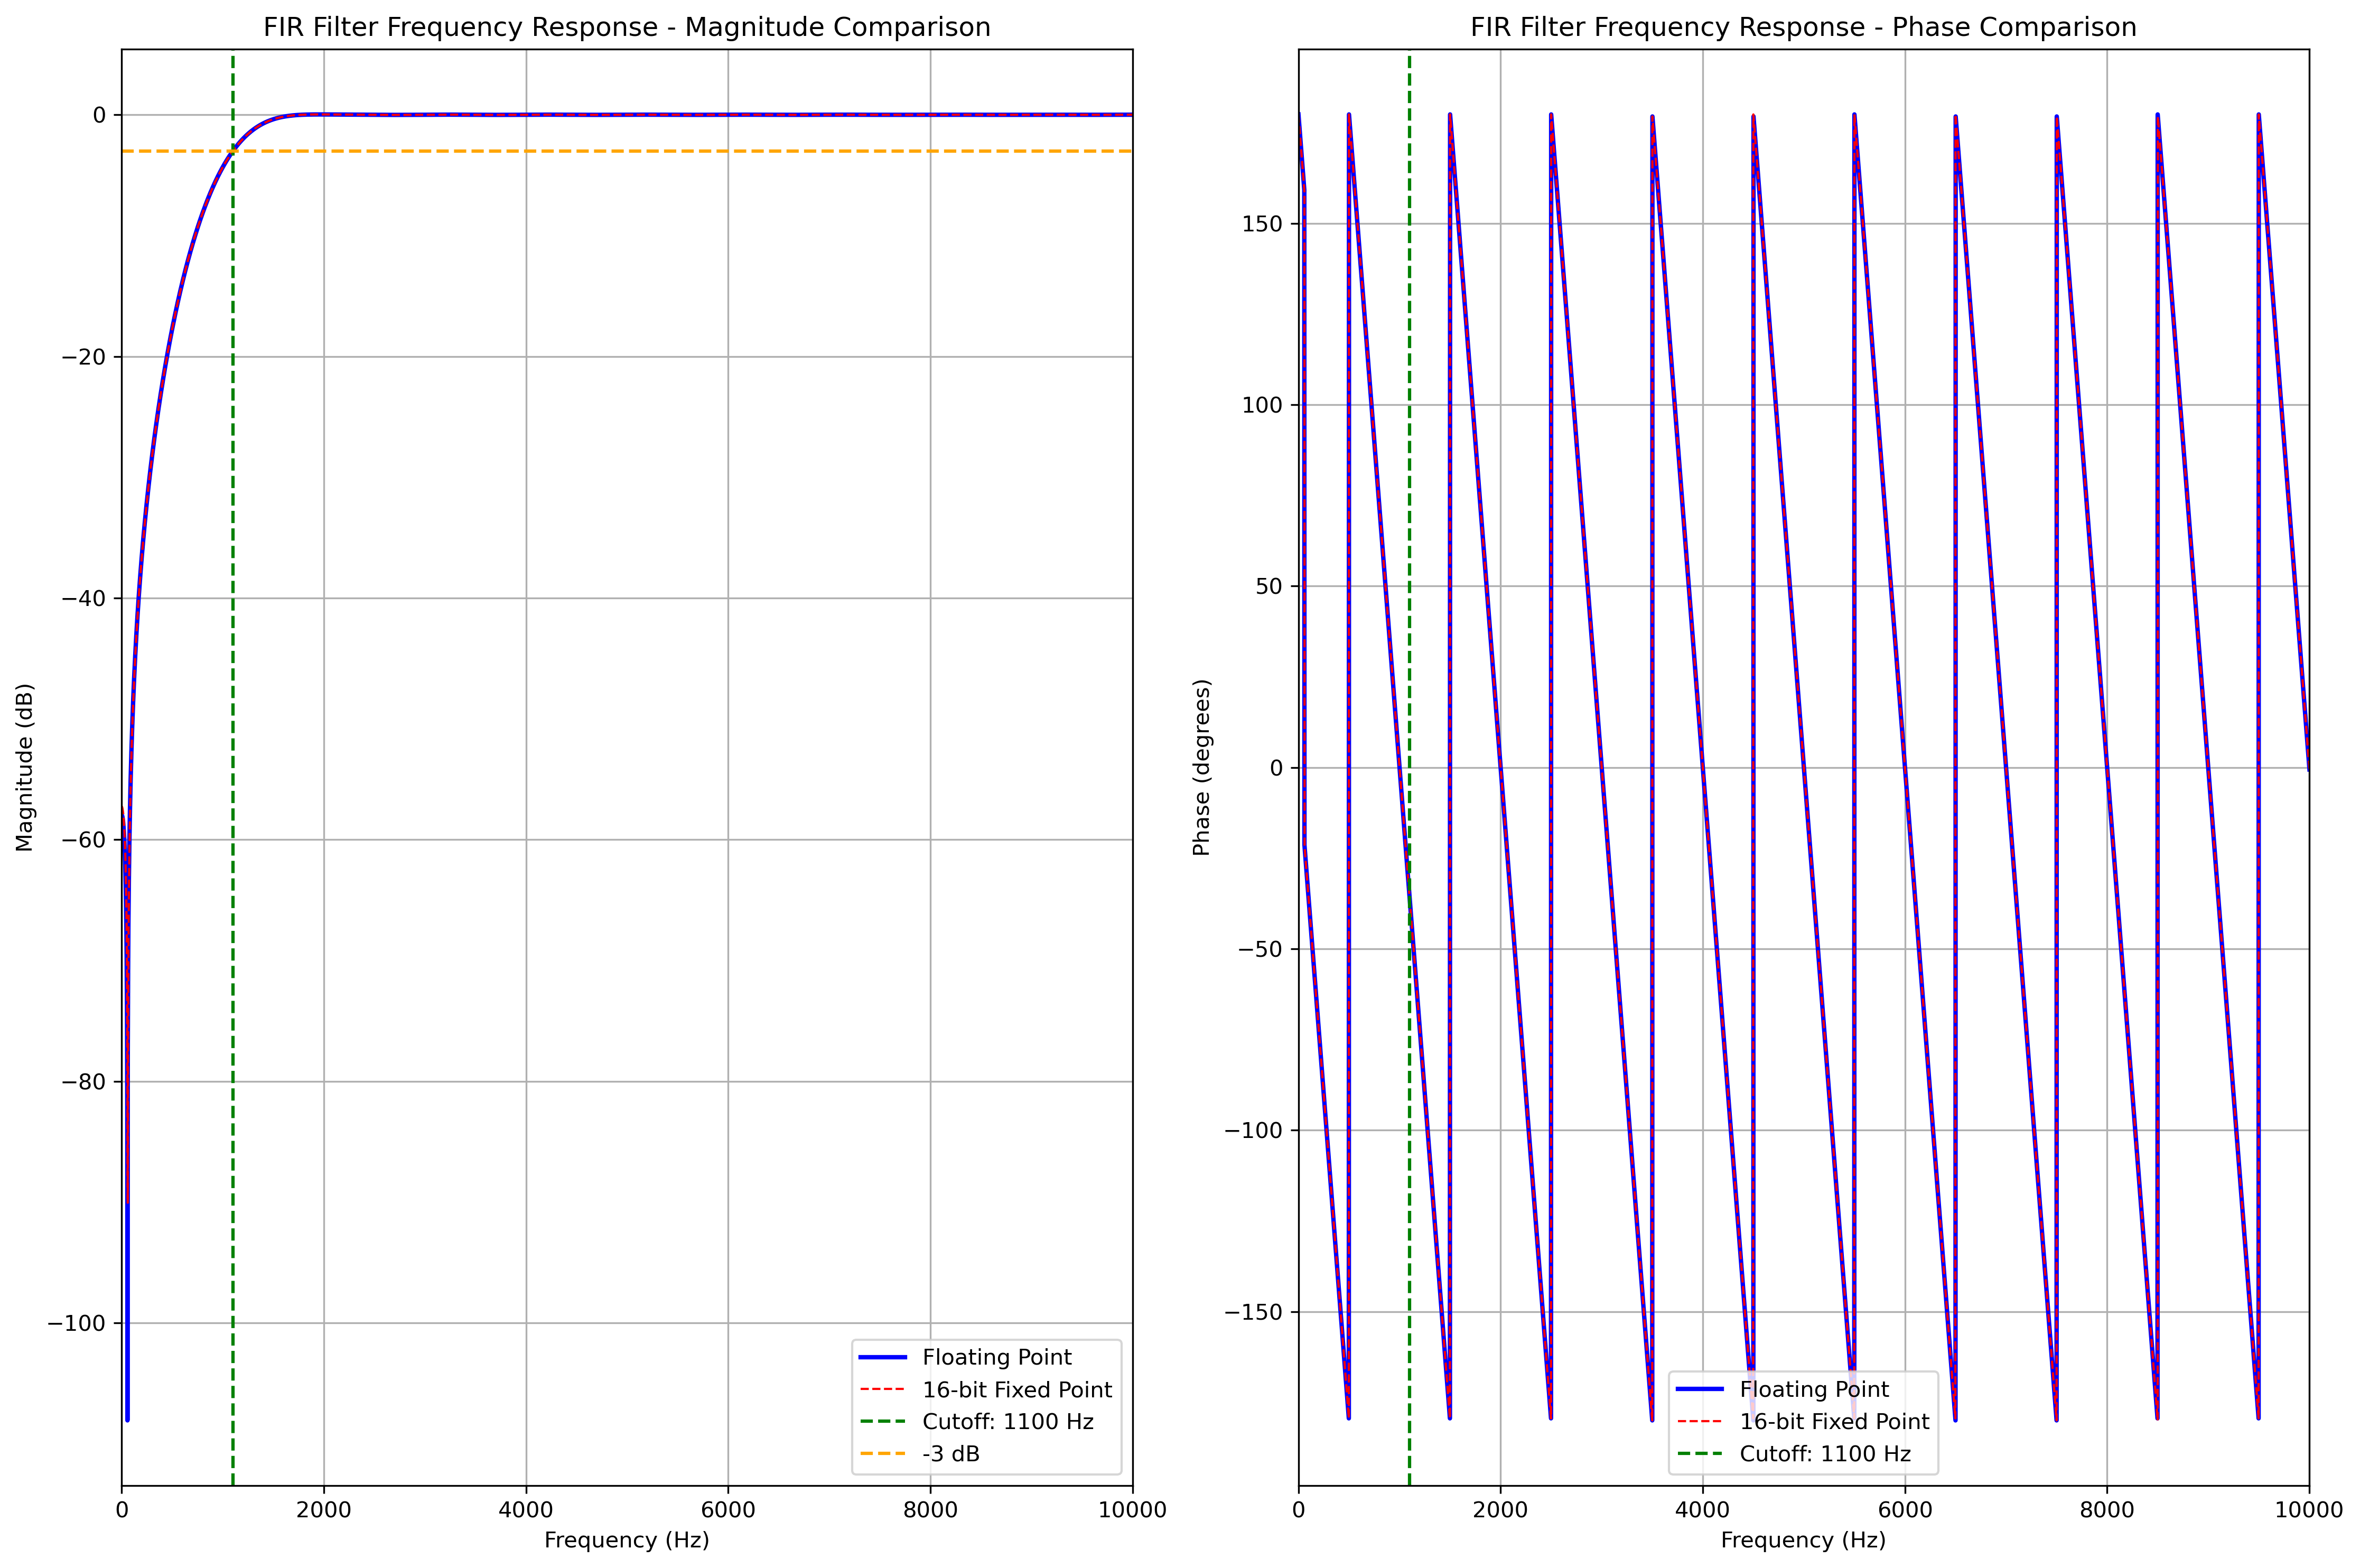
\includegraphics[width=0.8\textwidth]{fir_filter_response_16bit.png}
  \caption{Respon Frekuensi Filter FIR High-Pass}
  \label{fig:frequency_response}
\end{figure}

Hasil dari desain filter ini adalah koefisien filter dengan kuantisasi format fixed-point 16-bit,
agar dapat diimplementasikan pada FPGA. Koefisien yang dihasilkan adalah sebagai berikut:
\begin{table}[H]
  \centering
  \footnotesize
  \begin{tabular}{|c|c|c|c|c|c|c|c|c|c|c|}
    \hline
    h[0-9] & 0.000580 & 0.000824 & 0.001160 & 0.001556 & 0.002075 & 0.002625 & 0.003143 & 0.003510 & 0.003601 & 0.003204 \\
    \hline
    h[10-19] & 0.002167 & 0.000336 & -0.002411 & -0.006165 & -0.010956 & -0.016663 & -0.023224 & -0.030396 & -0.037903 & -0.045441 \\
    \hline
    h[20-29] & -0.052643 & -0.059143 & -0.064575 & -0.068726 & -0.071320 & \textbf{0.928253} & -0.071320 & -0.068726 & -0.064575 & -0.059143 \\
    \hline
    h[30-39] & -0.052643 & -0.045441 & -0.037903 & -0.030396 & -0.023224 & -0.016663 & -0.010956 & -0.006165 & -0.002411 & 0.000336 \\
    \hline
    h[40-49] & 0.002167 & 0.003204 & 0.003601 & 0.003510 & 0.003143 & 0.002625 & 0.002075 & 0.001556 & 0.001160 & 0.000824 \\
    \multicolumn{11}{|c|}{h[50] = 0.000580} \\
    \hline
  \end{tabular}

  \caption{Koefisien Filter FIR}
  \label{tab:fir_coeffs}
\end{table}
\begin{table}[H]
  \centering
  \footnotesize
  \begin{tabular}{|c|c|c|c|c|c|c|c|c|c|c|}
    \hline
    h[0-9] & 0x0013 & 0x001B & 0x0026 & 0x0033 & 0x0044 & 0x0056 & 0x0067 & 0x0073 & 0x0076 & 0x0069 \\
    \hline
    h[10-19] & 0x0047 & 0x000B & 0xFFB1 & 0xFF36 & 0xFE99 & 0xFDDE & 0xFD07 & 0xFC1C & 0xFB26 & 0xFA2F \\
    \hline
    h[20-29] & 0xF943 & 0xF86E & 0xF7BB & 0xF734 & 0xF6DF & \textbf{0x76D1} & 0xF6DF & 0xF734 & 0xF7BB & 0xF86E \\
    \hline
    h[30-39] & 0xF943 & 0xFA2F & 0xFB26 & 0xFC1C & 0xFD07 & 0xFDDE & 0xFE99 & 0xFF36 & 0xFFB1 & 0x000B \\
    \hline
    h[40-49] & 0x0047 & 0x0069 & 0x0076 & 0x0073 & 0x0067 & 0x0056 & 0x0044 & 0x0033 & 0x0026 & 0x001B \\
    \multicolumn{11}{|c|}{h[50] = 0x0013} \\
    \hline
  \end{tabular}
  \caption{Representasi Heksadesimal Koefisien Filter FIR}
  \label{tab:fir_coeffs_hex}
\end{table}
\subsection{Implementasi FIR VHDL}
Implementasi filter FIR pada VHDL menggunakan arsitektur direct-form dengan struktur shift register dan multiply-accumulate unit yang tersinkron dengan ADC (25 kHz).
Filter ini dirancang dengan 51 koefisien (tap) yang diimplementasikan menggunakan format fixed-point 16-bit Q15.

\begin{lstlisting}[style=vhdl, caption={Entity FIR Filter}]
ENTITY fir_filter IS
  PORT (
    clk : IN STD_LOGIC;
    reset_n : IN STD_LOGIC;
    sample_enable : IN STD_LOGIC;
    data_in : IN STD_LOGIC_VECTOR(11 DOWNTO 0);
    data_out : OUT STD_LOGIC_VECTOR(11 DOWNTO 0)
  );
END ENTITY fir_filter;
\end{lstlisting}

Arsitektur filter terdiri dari shift register yang menyimpan 51 sampel data input terakhir dalam array \texttt{taps},
dimana setiap kali sinyal \texttt{sample\_enable} aktif, data baru dimasukkan ke posisi pertama dan semua data lama
bergeser satu posisi ke kanan. Input ADC 12-bit unsigned dikonversi menjadi signed dengan mengurangi offset DC
sebesar 2048 untuk memastikan pemrosesan aritmatika yang dalam domain signed.

Unit multiply-accumulate (MAC) melakukan operasi perkalian dan akumulasi secara paralel untuk semua 51 tap,
dimana setiap tap data dikalikan dengan koefisien yang sesuai dan semua hasil perkalian dijumlahkan untuk
menghasilkan output filter.
Operasi MAC ini diimplementasikan secara parallel atau kombinatorial.

Tahap akhir melakukan scaling output dimana hasil
akumulasi 28-bit di-scale down menjadi 12-bit dengan mengambil bit [26:15],
kemudian ditambahkan kembali offset DC sebesar 2048 untuk menghasilkan output unsigned yang kompatibel dengan format ADC.

\subsection{Komunikasi UART}

\begin{lstlisting}[style=vhdl, caption={Entity UART Transmitter}]
ENTITY UART_TX IS
  GENERIC (
    g_CLKS_PER_BIT : INTEGER := 17 -- #3Mbaudps at 50MHz clock
  );
  PORT (
    i_Clk : IN STD_LOGIC;
    i_TX_DV : IN STD_LOGIC;
    i_TX_Byte : IN STD_LOGIC_VECTOR(7 DOWNTO 0);
    o_TX_Active : OUT STD_LOGIC;
    o_TX_Serial : OUT STD_LOGIC;
    o_TX_Done : OUT STD_LOGIC
  );
END UART_TX;
\end{lstlisting}

Modul UART transmitter digunakan untuk mengirimkan data hasil filtering dan raw ke komputer dengan baudrate 3 Mbps.
Modul ini mengimplementasikan protokol UART standar dengan 8 bit data, 1 start bit, 1 stop bit, dan tanpa parity bit.
Sistem utama mengirimkan frame data yang terdiri dari header (0xAE, 0xBC) untuk sinkronisasi diikuti dengan data ADC dan hasil filter yang
masing-masing dikemas dalam 2 byte untuk mempertahankan resolusi 12-bit.

\subsection{Implementasi Python untuk Visualisasi Data}
Aplikasi Python dikembangkan untuk visualisasi real-time data ADC dan hasil filtering menggunakan library matplotlib,
serial, dan threading. Program ini mengimplementasikan parser protokol komunikasi UART dengan
finite state machine untuk memproses frame data yang diterima dari FPGA.

Arsitektur aplikasi menggunakan multi-threading dimana thread utama menangani GUI matplotlib sedangkan
thread terpisah membaca data serial secara kontinyu. State machine parser mengidentifikasi header frame (0xAE, 0xBC)
kemudian mengekstrak 4 byte data yang merepresentasikan nilai ADC channel 0 dan channel 1 dalam format 12-bit.
Data yang diterima disimpan dalam queue thread-safe untuk komunikasi antar thread.

Visualisasi menggunakan dua subplot yang menampilkan sinyal ADC asli dan hasil filtering secara real-time dengan
buffer circular berukuran 500 sampel. Setiap subplot dilengkapi dengan statistik peak-to-peak.
Update plot dilakukan setiap 50ms menggunakan FuncAnimation matplotlib untuk mempertahankan responsivitas GUI sambil menampilkan data pada frekuensi sampling 25 kHz.

\newpage
\section{Hasil Percobaan}
Rangkaian percobaan diuji seperti
pada gambar dibawah. Function generator
digunakan untuk
menghasilkan sinyal sinus
untuk ADC FPGA. FPGA mengfilter dan mengirim data
filter dan raw ke komputer dengan komunikasi UART, melalui USB-TTL CH340.

\begin{figure}[H]
\centering
\begin{subfigure}{0.45\textwidth}
    \centering
    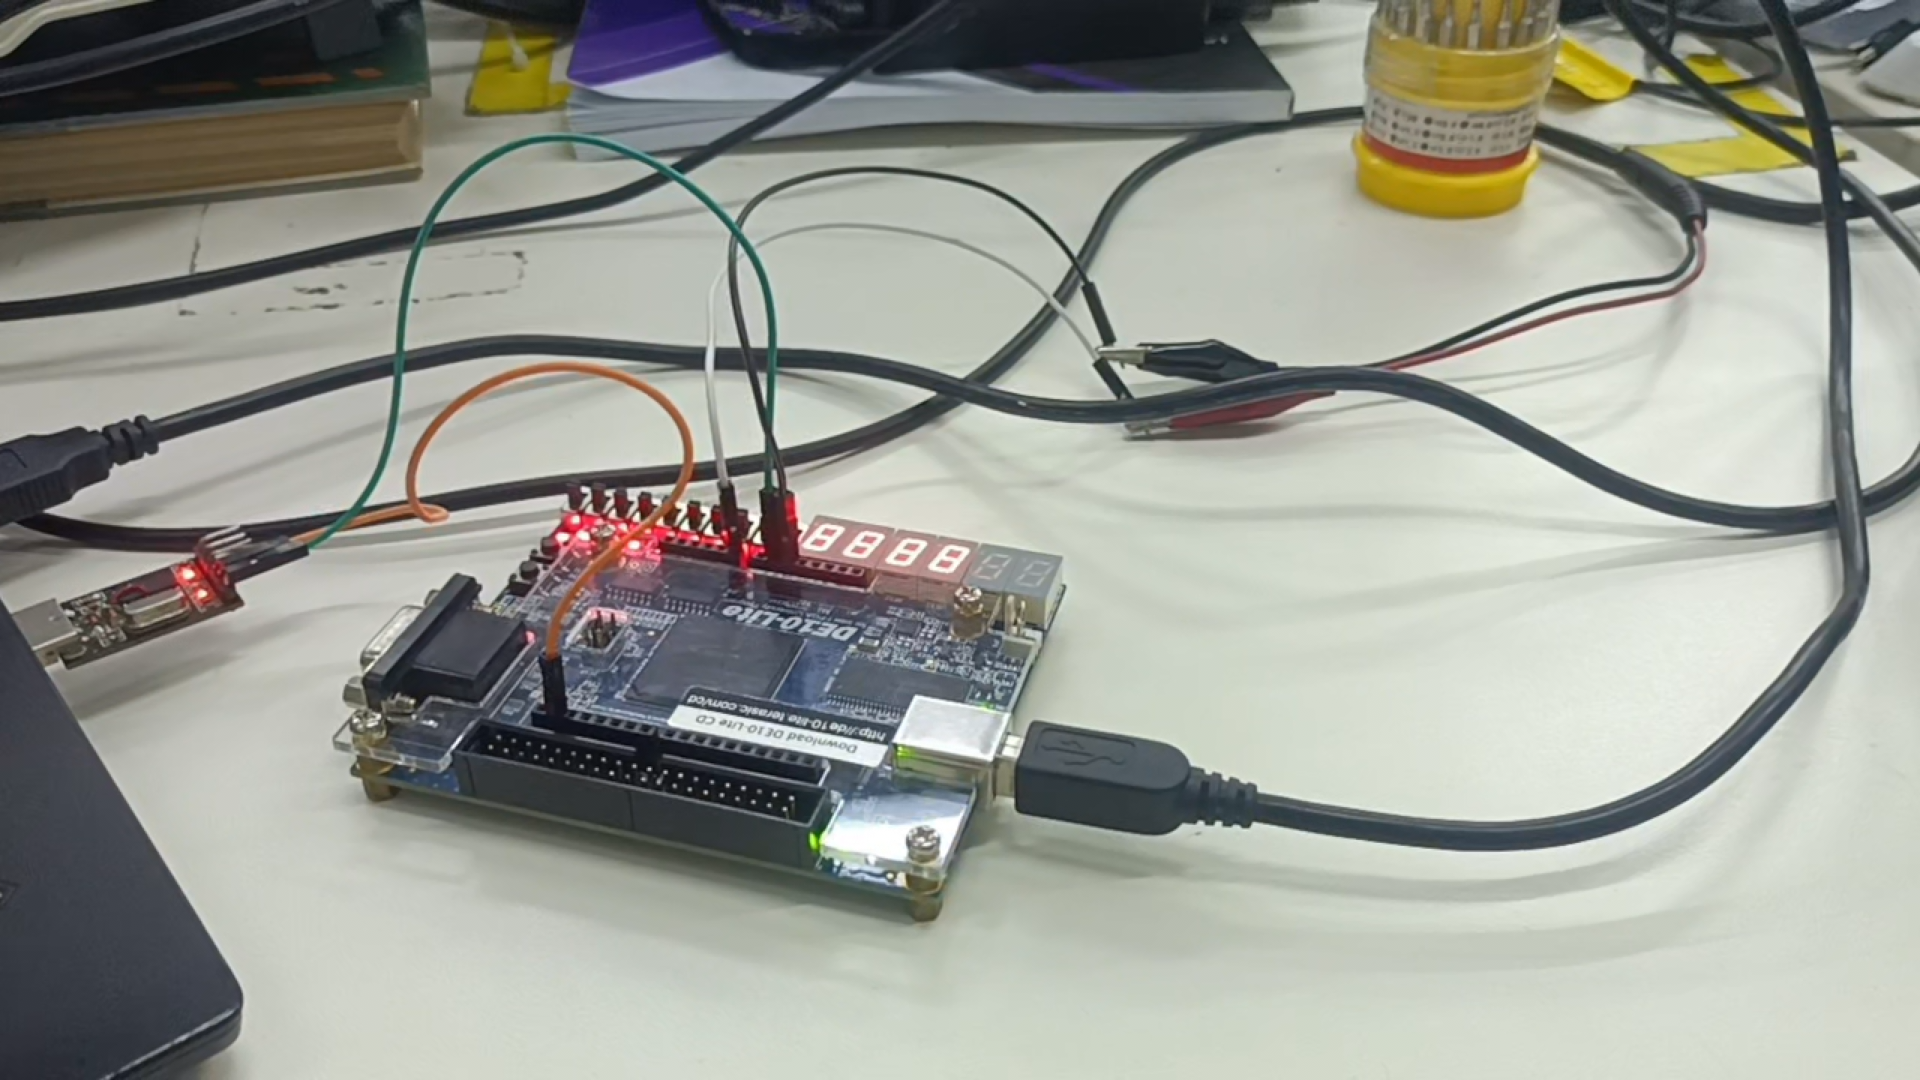
\includegraphics[width=\textwidth]{setup.png}
    \caption{Setup eksperimen dengan FPGA DE-10 Lite, USB-TTL CH340, dan function generator}
    \label{fig:setup}
\end{subfigure}
\hfill
\begin{subfigure}{0.45\textwidth}
    \centering
    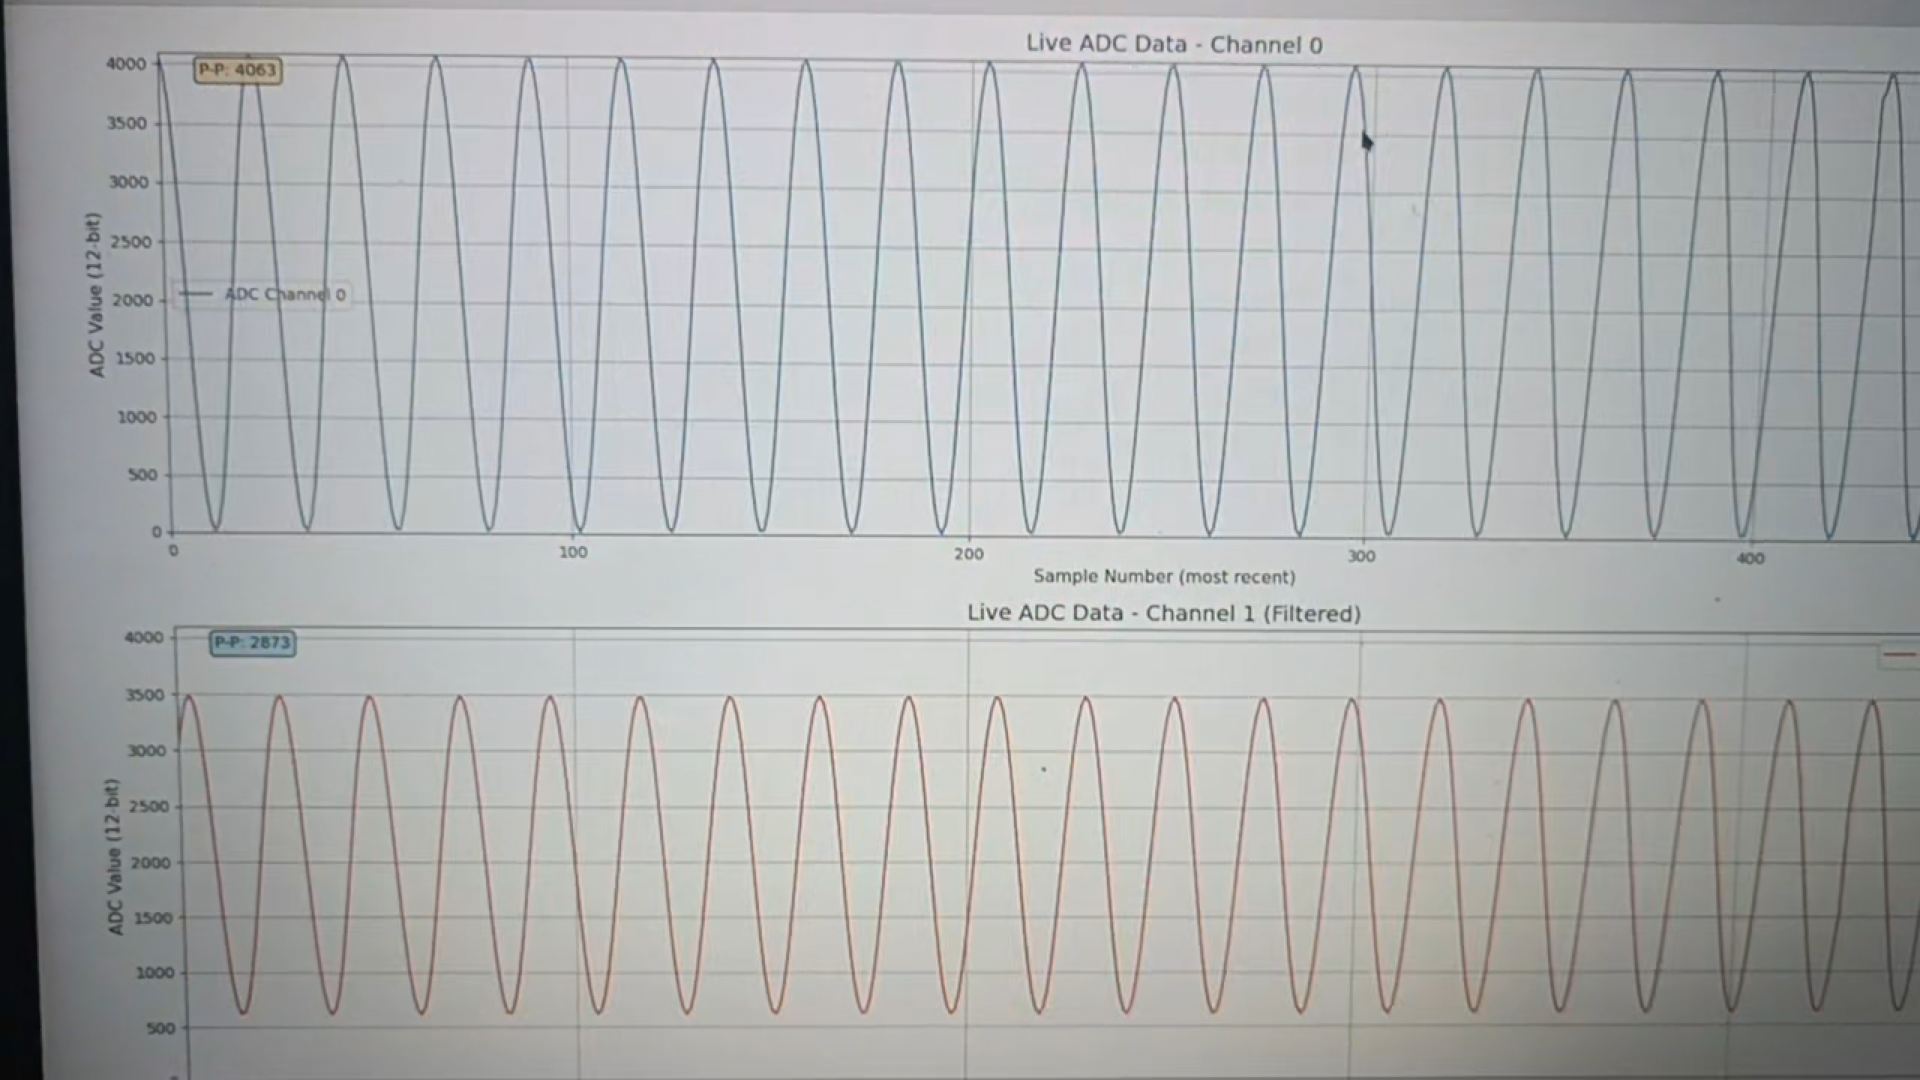
\includegraphics[width=\textwidth]{cutoff.png}
    \caption{Respons filter pada frekuensi cut-off 1.1 kHz (output = 0.707 × input)}
    \label{fig:cutoff}
\end{subfigure}

\vspace{0.5cm}

\begin{subfigure}{0.45\textwidth}
    \centering
    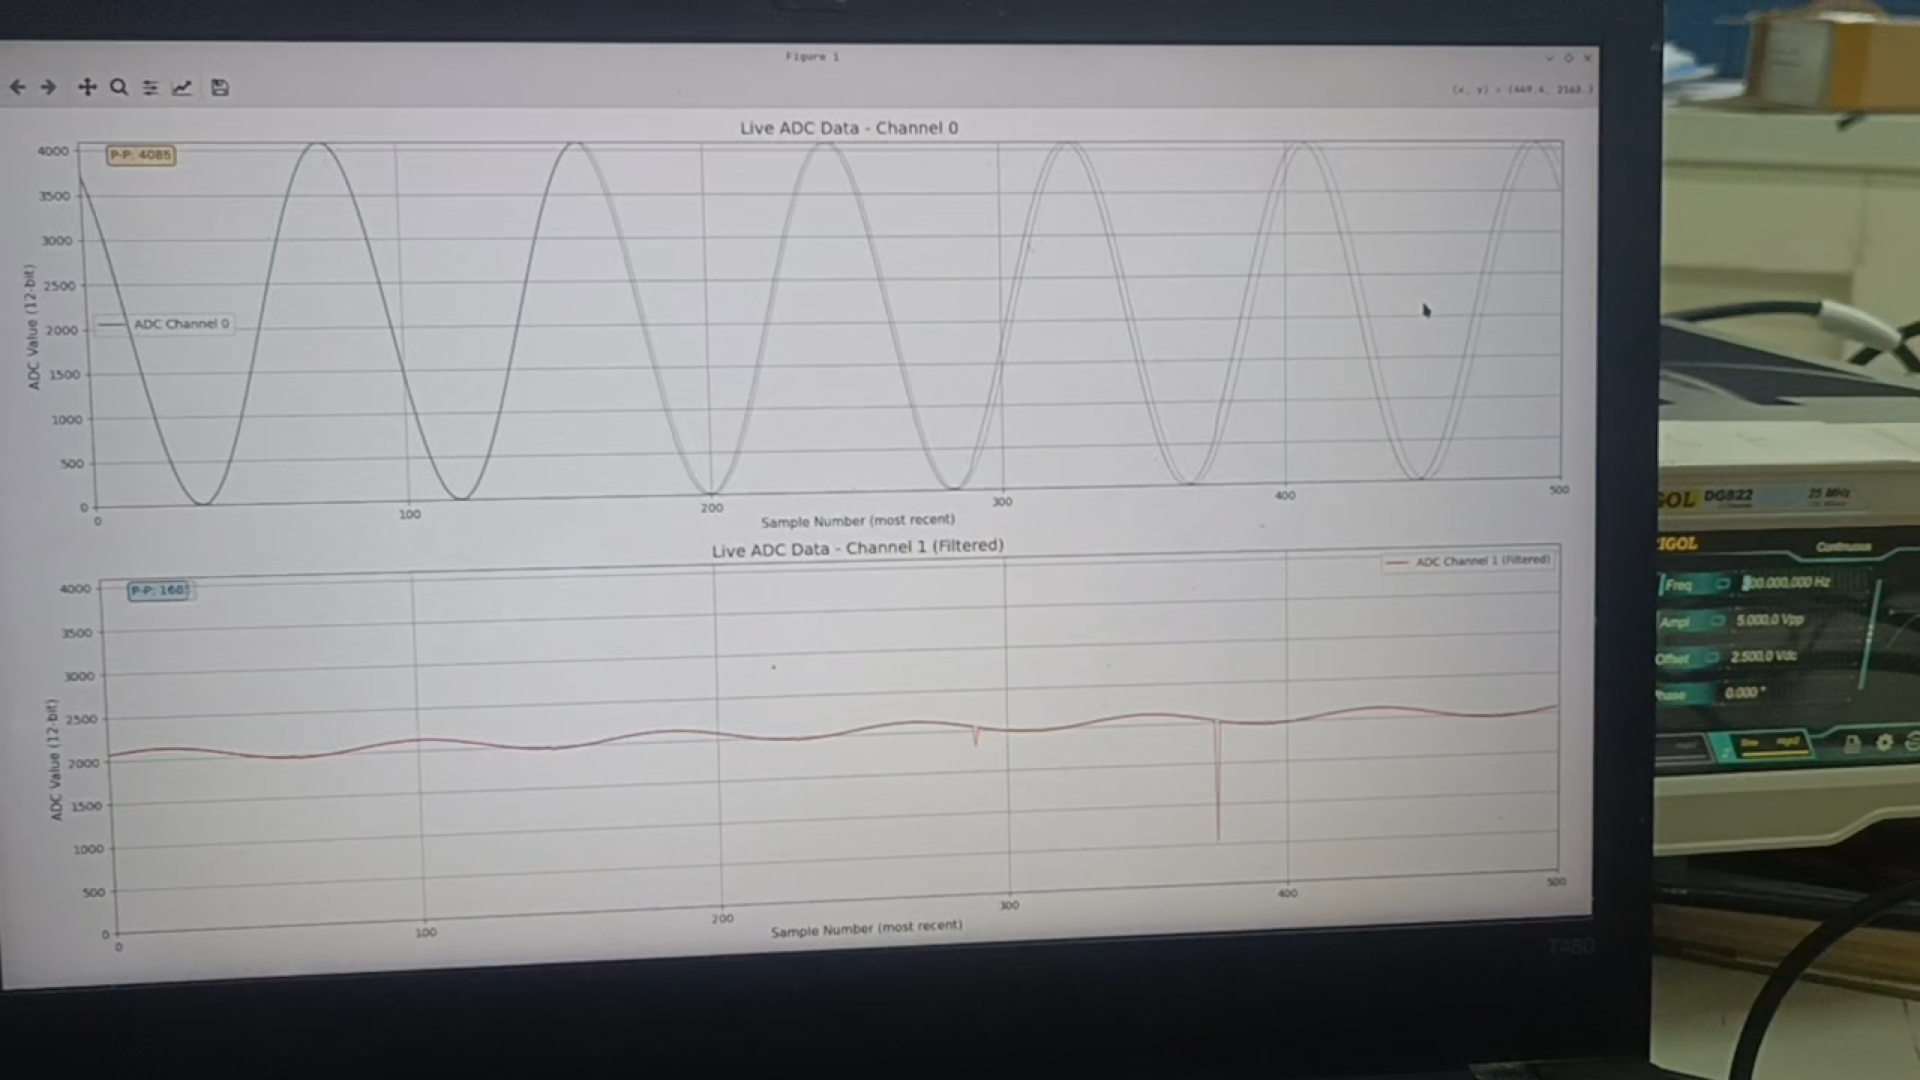
\includegraphics[width=\textwidth]{300Hz.png}
    \caption{Respons filter pada 300 Hz (output sangat kecil, frekuensi diredam)}
    \label{fig:300hz}
\end{subfigure}
\hfill
\begin{subfigure}{0.45\textwidth}
    \centering
    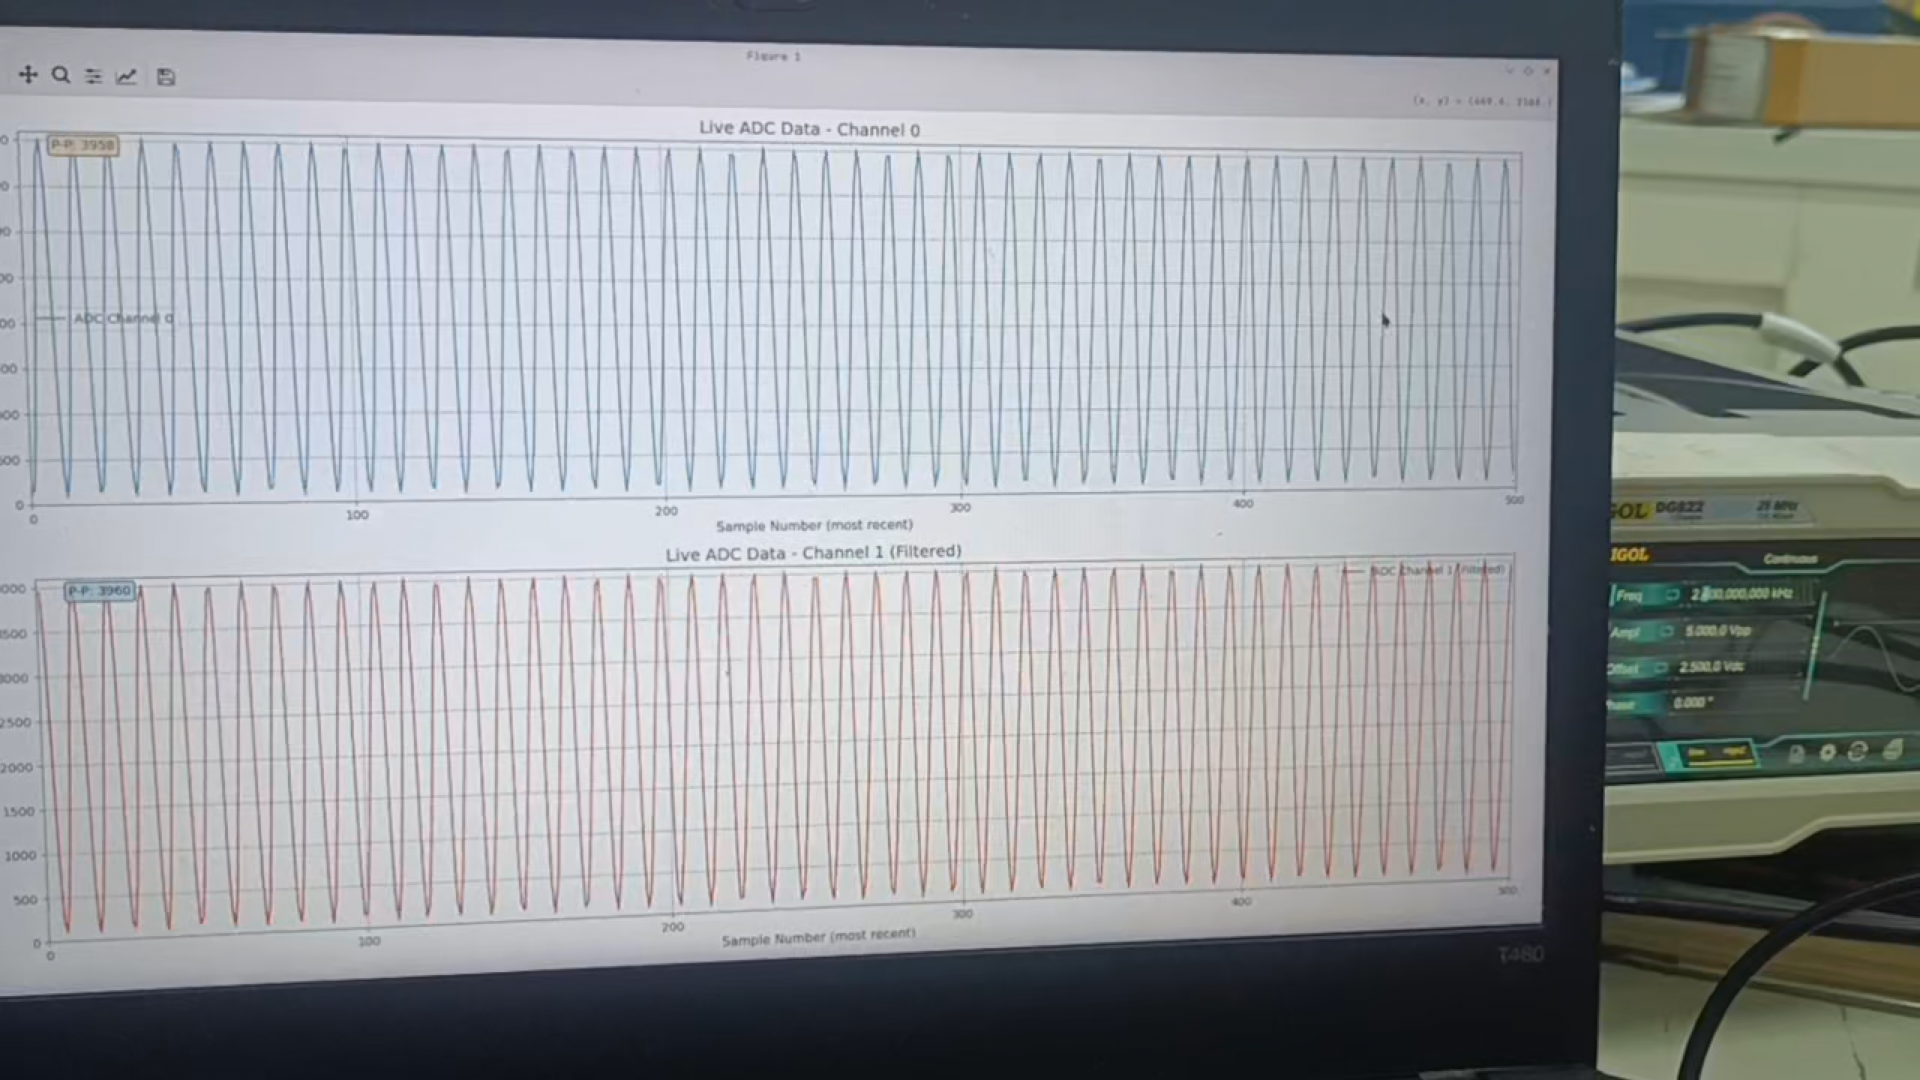
\includegraphics[width=\textwidth]{2k5Hz.png}
    \caption{Respons filter pada 2.5 kHz (output = input, frekuensi diloloskan)}
    \label{fig:2k5hz}
\end{subfigure}

\caption{Hasil pengujian filter FIR high-pass pada berbagai frekuensi}
\label{fig:results}
\end{figure}

\end{document}